\documentclass[10pt]{article}
\usepackage[margin=1in]{geometry}
\usepackage{multicol}
%\usepackage{setspace}
%\usepackage{amstext}
%\usepackage{amsmath}
%\usepackage{enumerate}
\usepackage{graphicx}
\usepackage{wrapfig}

\title{
	\textbf{
		Creating a Turn-Based Conflict Resolution Simulator FIX TEAMS INVADING A NODE
	}
}
\author{Noah Zimmt and Dakota Szabo}
\date{May 8, 2012}

\begin{document}
	\maketitle
	\begin{abstract}
		In this paper, we describe a territory-conquest simulation modeled on the classic board game \emph{RISK} and present a parallelized method for efficiently simulating multiple rounds of the model. 
		Players compete on a gameboard represented by an undirected graph, with vertices and edges representing territories and their borders, respectively. 
		Using MPI, we distributed the computation and resolution of player actions between multiple compute nodes in order to acheive the speed neccessary to simulate massive games in a reasonable amount of time. 
		This was acheived via a randomized algorithm that partitioned the computational work between nodes, combined with by a pair of message-passing cycles that communicated the results of the computations to each node. 
		In performance testing, we found this method to scale reasonably with the size of the input graph, with expected variation depending on the graph shape (complete graphs performing better than stars, etc).
	\end{abstract}

	\begin{multicols}{2}
		\section*{Introduction}
		
		Our simulation is designed as a territory-conquest simulator, with multiple teams competing against one another to dominate the entirety of the gameboard. 
		The gameboard itself is laid out as an undirected graph in which territories correspond to vertices and borders between territories correspond to edges.
		Each territory has a troop count, representing the number of soliders currently stationed in that territory, as well as a team affiliation, representing the team currently controlling it.
		Gameplay consists of a series of turns, each with two stages. 
		During the troop placement stage, each territory determines how many troops from its army to place on each of its borders.
		Troops placed on a border with another territory may either be attacking that territory or defending against an attack.
		After all troops have been placed, the game proceeds to the conflict resolution stage.
		Along every edge of the graph (every border between territories), a battle takes place if at least one of the territories chose to attack during the placement stage (if both teams defend, no battle takes place and all troops survive).
		Battles are resolved in the following fashion: 
		Territories flip a number of coins depending on the action they chose (attack or defend) and the amount of troops they have stationed on the edge where the battle is taking place. 
		Attacking territories flip one coin per solider; defending territories flip two coins per solider.
		After all coins are flipped, the number of heads for each side is tallied and subtracted from the number of opposing soliders on that edge (each coin flip is a gunshot; each heads is a successful hit and kill).
		This coin flipping process repeats until one or both territories have no further soliders remaining on that edge. 
		After all battles are resolved, surviving attacking troops proceed into the territory they were attacking, while defending troops retreat back to the territory they were defending. 
		The team with the largest number of troops present in a given territory after the battle phase becomes the new owner of that territory, and troops from other teams currently occupying the territory are considered killed.
		Territories are then given a 'recruitment bonus' (a number of troops added to their troop count) depending on their current troop count - this is currently 20 percent but is easily configurable within the rules of the game.
		The turn is then considered completed, and the game proceeds back to the troop placement stage.
		The game ends if, at the end of a turn, one of three conditions is met. 
		If every territory is controlled by a single team, that team is considered the winner. 
		Likewise, if only one team still has troops remaining on the board (territories may lose all troops but remain unconquered), it is considered the winner.
		Finally, if no troops remain on the board, the game is considered a draw and the gameboard begins recovering from the armageddon that has transpired (for the sake of this simulation, we do not model the reconstruction of humanity).

		\section*{Implementation}
		To process events in parallel, each compute node must have a subset of the data used to represent the entire simulation.  
		Because the total amount of data being stored for the entire simulation grows exponentially with the size of the input graph, we partition the graph into sets of vertices, with each compute node being responsible for a given slice of the graph.  
		A compute node stores the team, total troop count, battle decisions, and battle resolutions for each of its vertices.
		Because each battle is fought over an edge, and an edge may connect two vertices whose data is contained on two different compute nodes, we elect a single compute node to be responsible for the battle that takes place on any given edge of the graph.
		Being that edge-coloring is known to be an NP-Complete problem, we devised an approximate solution for assigning battle computation to each compute node such that the work was resonable evenly distributed across all compute nodes: each territory flips a coin at the start of its turn; upon entering a battle, the coin flips are compared.  
		If the coin flips are the same, the compute node whose territory has a lower ID number is responsible for the calculation; otherwise, the other compute node is responsible.

		Our parallelized simulation models each game round in two main stages: an edge conflict stage and an internal vertex conflict stage.
		First, the edge conflict resolution stage determines and computes the outcomes of all battles that occurred during the round, with each battle taking place on an edge (a border between territories). 
		Because of the graph partitioning scheme, it was necessary to communicate a territory's battle stances to each of its bordering territories.  
		We did this using a round-robin inter-node communication method that enabled us to pass slices of a larger matrix of battle information to each node in turn; each compute node would scan the slice of battle data that it received, taking note of any important information about bordering territories engaging in battles with any of its territories.  
		Once all information was passed around, each compute node had enough information to compute the results for its share of battles for the turn (our coin-flip algorithm ensures that no computation is performed redundantly).  
		At this point in the turn, all battle information is decided. 
		To communicate this information back to the territories that it affects, we again utilize a round-robin data passing scheme that we refer to as the \emph{report card scheme}: each compute node creates and fills in a report card about all territories for which it is responsible.
		Each compute node then passes its report card to its right-hand neighbor (for the sake of simplicity, we visualize the compute nodes in a circular arrangement).  
		The neighbor then fills in information that it had computed about the first compute node's territories and passes the report card to its right. 
		This process continues until the report card arrives back at its owner, ensuring that at the end of the round-robin, each compute node's report card will have been filled in by each of the other compute nodes.
		
		Next, the internal vertex conflict resolution stage uses the data from the edge-conflict phase to decide which territories were conquered by which teams. 
		After all battles and takeovers are resolved, each compute node computes the total remaining number of troops in each territory and then decides which team now owns each territory that it is responsible for.
		At this point, each compute node has a new set of data about each of its territories; critical data such as team membership, total troop counts, and new coin flips for battle computation are distributed from each compute node to each other compute node via AllReduce.
		
		\section*{Performance Analysis}
		
		\begin{center}
			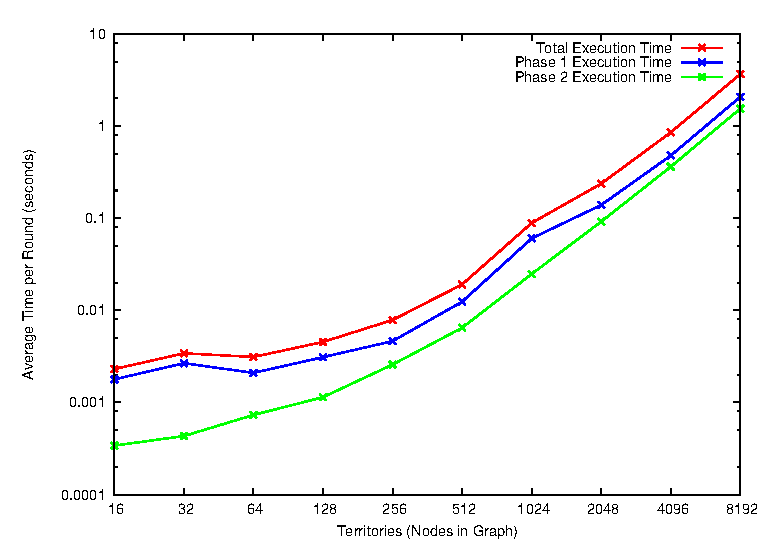
\includegraphics[width=.45\textwidth]{graphs.eps}
			%\vspace*{-10pt}
			\small{Figure 1: Herpaderp}
		\end{center}
		
		\begin{center}
			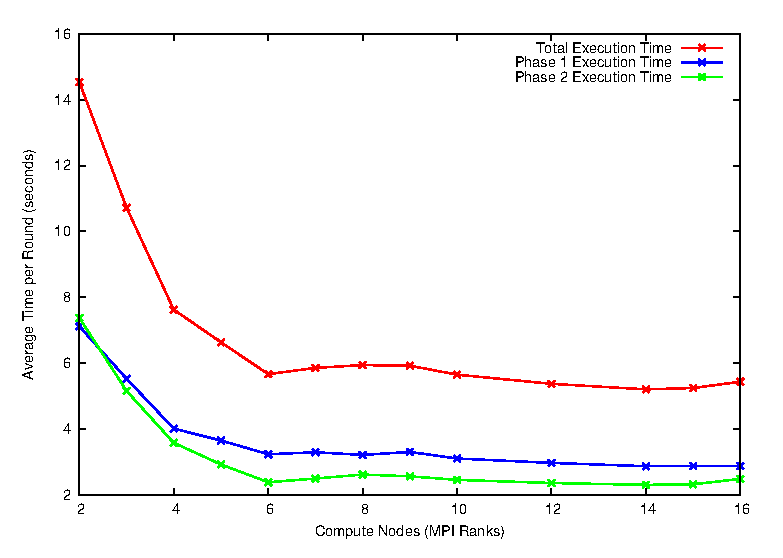
\includegraphics[width=.45\textwidth]{ranks.eps}
			%\vspace*{-10pt}
			\small{Figure 2: Herpaderpa}
		\end{center}
		
		Proin scelerisque urna et velit rutrum non feugiat nibh luctus. Aliquam posuere viverra lectus ut varius. Nam at erat tellus. Donec sed consectetur felis. Praesent at justo sit amet est vehicula pharetra viverra et magna. Nulla dignissim consectetur facilisis. Vestibulum a dui ligula. Nullam ornare sollicitudin molestie. Integer fringilla lacus ut metus lobortis mollis. Fusce magna velit, pulvinar a molestie vel, cursus et lorem. Phasellus semper pellentesque turpis eget faucibus. Proin at neque eu neque elementum sollicitudin vitae sit amet nunc. Etiam nec erat ut enim sagittis facilisis. Curabitur sollicitudin convallis arcu sit amet dignissim. Pellentesque habitant morbi tristique senectus et netus et malesuada fames ac turpis egestas.
		



		
		\section*{Conclusion}
		Nullam tortor mi, volutpat quis auctor non, aliquam id tellus. Morbi a massa libero, id tempus mi. Aliquam et sapien non est mollis interdum. Cras felis diam, luctus eget pellentesque ut, lacinia nec dui. Aenean eu orci neque, eu volutpat enim. Sed eleifend fringilla turpis, sed pharetra libero mollis non. Quisque ultrices, purus ut sagittis euismod, orci risus venenatis lacus, a auctor diam augue vitae dolor. Duis eleifend pulvinar enim ac mollis. Nulla auctor metus vel turpis consequat aliquam.
		

		\section*{Related Work}
		Graph partitioning is a well-studied problem.  Our simulator used a trivial graph partitioning algorithm to divide up nodes among compute nodes.  Karypis and Kumar (IEEE HPC 1998) describe a parallel graph paritioning algorithm that promises high-performance partitioning with constraints on the partitioning schemes used.  In addition to graph partitioning, the distribution of computation among compute cores can be reduced to a variant of the NP-Complete edge-coloring problem as described by Holyer (Society for Industrial and Applied Mathematics, 1981); approximation algorithms exist to achieve a near-optimal solution (as described by Sanders and Steurer, ACM TALG, 2008).

		\section*{Future Work}
		 - Further modularization of team strategy?
		 - Scaling studies on BlueGene/L \& BlueGene/Q
		 - Optimization of graph partitioning and/or calculation distribution
		 - Graph visualization for higher territory counts.
		 - Experiments with different graph shapes/type and effects on performance



	\end{multicols}
\end{document}


%George Karypis and Vipin Kumar. 1998. Multilevel algorithms for multi-constraint graph partitioning. In Proceedings of the 1998 ACM/IEEE conference on Supercomputing (CDROM) (Supercomputing '98). IEEE Computer Society, Washington, DC, USA, 1-13.

